
\documentclass[10pt]{article}
\usepackage[utf8]{inputenc}
\usepackage{graphicx}
\usepackage{amsmath, amssymb}
\usepackage{geometry}
\usepackage{caption} 
\geometry{a4paper, margin=0.5in, landscape} 

\begin{document}

\section*{Comparative EIS Kinetics Report}
\textbf{Model Structure:} \texttt{R0-p(R1-p(R2-Wo2,CPE2),CPE1)}

\begin{center}
    \includegraphics[width=0.45\textwidth]{circuit_2RC_Wo.png}
\end{center}

\renewcommand{\arraystretch}{1.6} 
\begin{table}[h!]
    \centering
    \footnotesize
    \begin{tabular}{|l|c|c|c|c|c|}
        \hline
        \textbf{Element} & \textbf{Unit} & \textbf{Bounds} & \textbf{Cauvel\_3\_BTA\_48H} & \textbf{Cauvel\_3\_BTA\_72H} & \textbf{Cauvel\_3\_BTA\_168H} \\ \hline
        $R_{0}$ & $\Omega$ & $[1.0e-03, 1.0e+03]$ & $8.20e+01 \pm 2.7e-01$ & $8.64e+01 \pm 2.4e-01$ & $8.45e+01 \pm 2.3e-01$ \\ \hline
        $R_{1}$ & $\Omega$ & $[1.0e+00, 1.0e+08]$ & $8.74e+03 \pm 3.2e+02$ & $7.91e+03 \pm 1.6e+02$ & $4.33e+03 \pm 6.0e+01$ \\ \hline
        $R_{2}$ & $\Omega$ & $[1.0e+00, 1.0e+08]$ & $4.12e+04 \pm 6.1e+03$ & $3.23e+04 \pm 4.6e+03$ & $2.17e+04 \pm 3.1e+03$ \\ \hline
        $W_{2,R}$ & $\Omega$ & $[1.0e-03, 1.0e+04]$ & $2.70e+03 \pm 1.6e+04$ & $2.15e+03 \pm 1.2e+04$ & $1.53e+03 \pm 8.1e+03$ \\ \hline
        $W_{2,\tau}$ & sec & $[1.0e+00, 1.0e+08]$ & $4.67e+00 \pm 2.7e+01$ & $4.77e+00 \pm 2.7e+01$ & $4.88e+00 \pm 2.6e+01$ \\ \hline
        $Q_{2}$ & $\Omega$$^{-1}$ sec$^{a}$ & $[1.0e-09, 1.0e-03]$ & $2.13e-05 \pm 1.3e-06$ & $3.77e-05 \pm 1.7e-06$ & $7.67e-05 \pm 2.7e-06$ \\ \hline
        $n_{2}$ & - & $[5.0e-01, 1.0e+00]$ & $8.70e-01 \pm 3.0e-02$ & $8.39e-01 \pm 2.2e-02$ & $7.83e-01 \pm 1.5e-02$ \\ \hline
        $Q_{1}$ & $\Omega$$^{-1}$ sec$^{a}$ & $[1.0e-09, 1.0e-03]$ & $1.18e-05 \pm 2.0e-07$ & $1.11e-05 \pm 1.4e-07$ & $1.13e-05 \pm 1.5e-07$ \\ \hline
        $n_{1}$ & - & $[5.0e-01, 1.0e+00]$ & $8.59e-01 \pm 2.5e-03$ & $8.63e-01 \pm 1.9e-03$ & $8.61e-01 \pm 2.0e-03$ \\ \hline
        \textbf{$\chi^2$} & - & -  & $4.331e-04$ & $3.076e-04$ & $2.897e-04$ \\ \hline

    \end{tabular}
\end{table}


\newpage
\section*{Analysis Results: 48H}
\begin{center}
    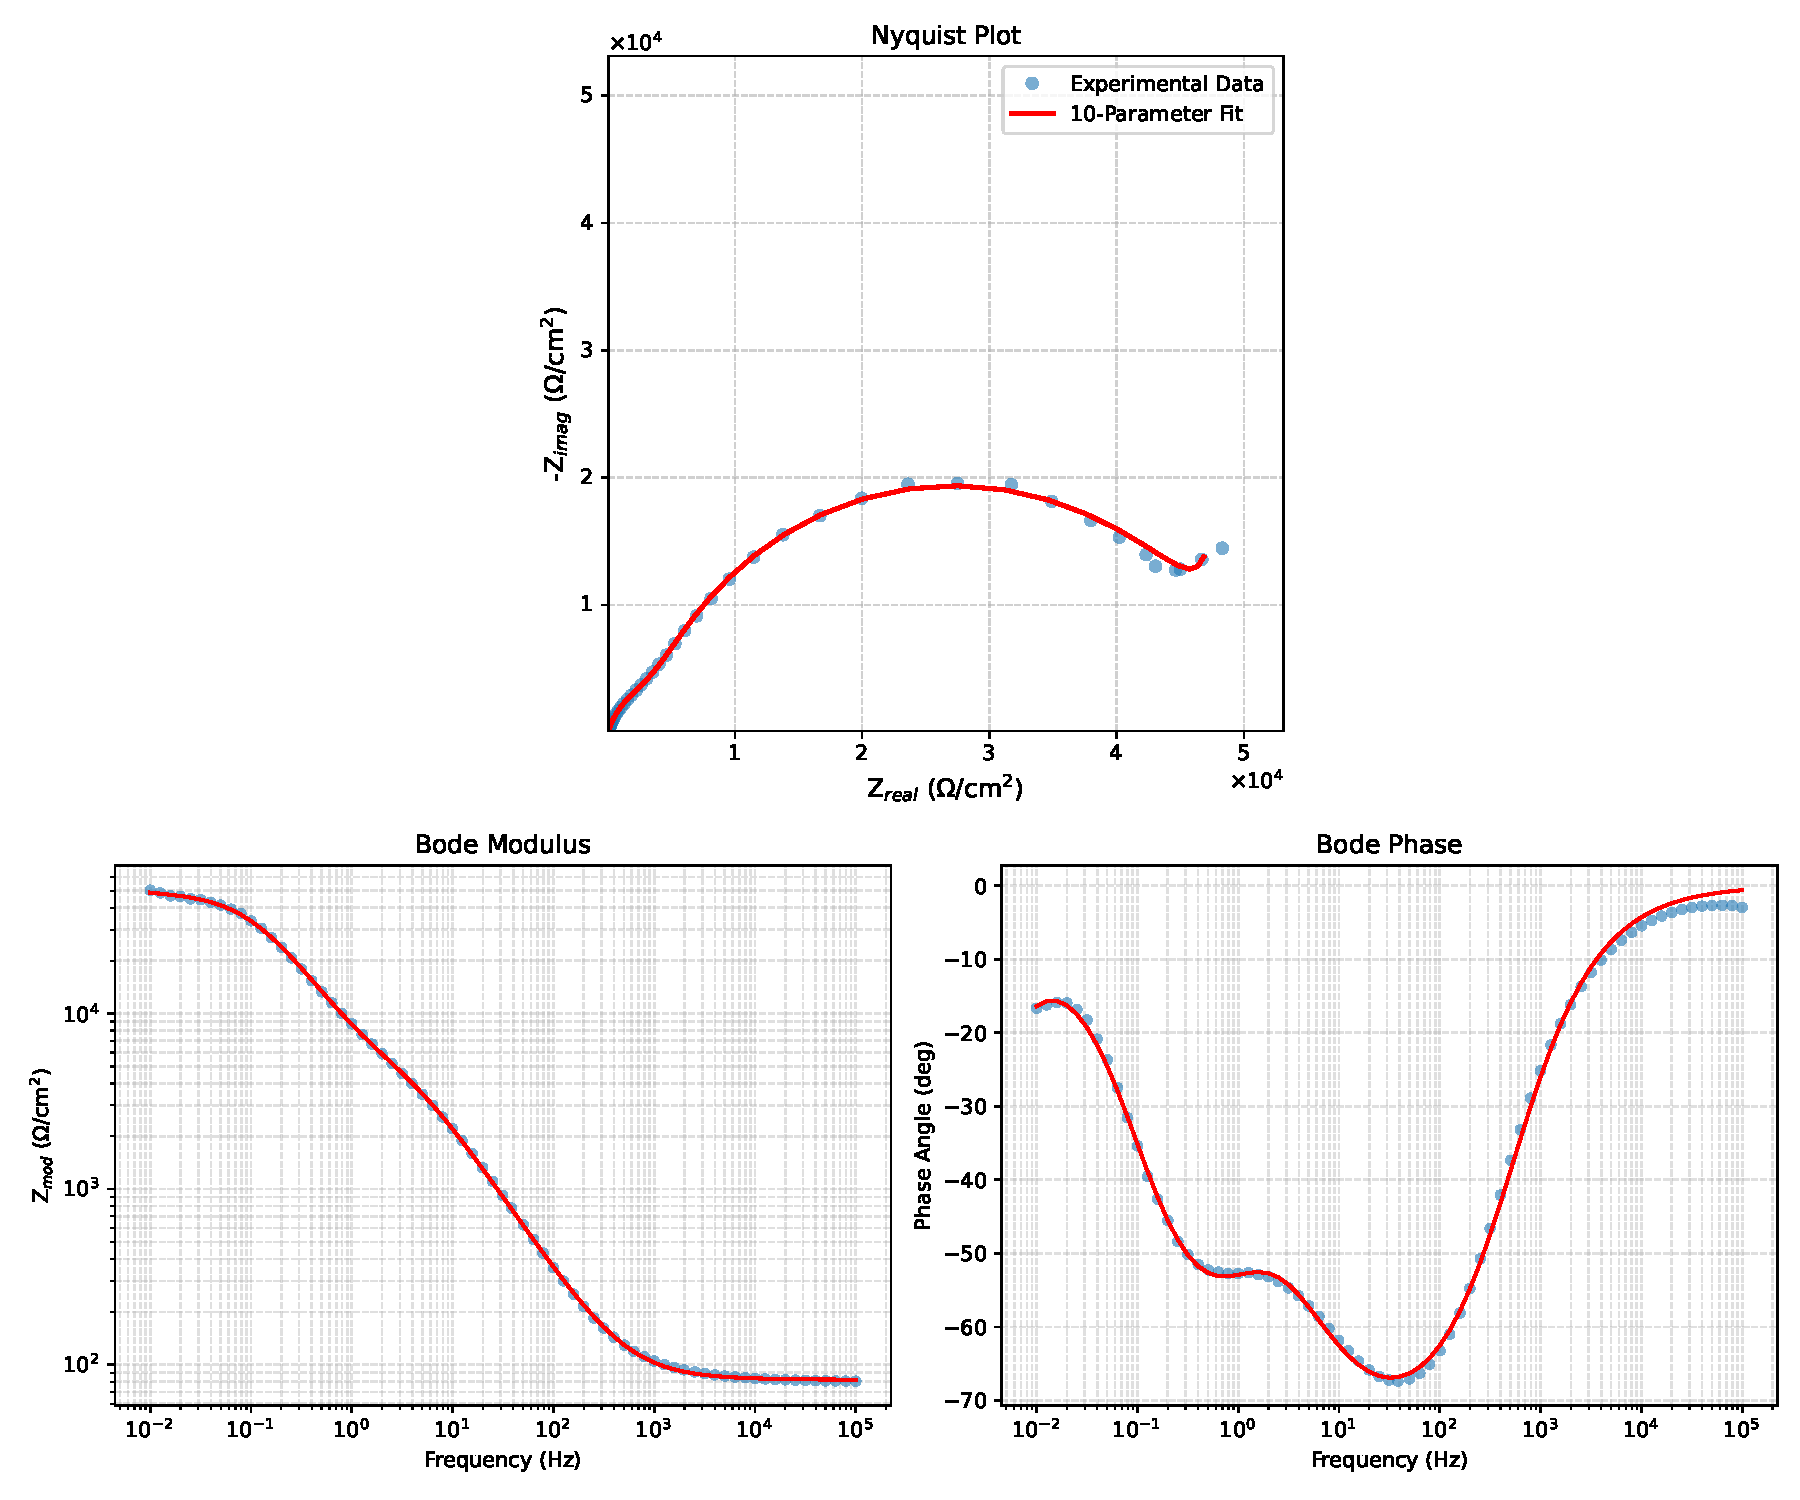
\includegraphics[width=0.7\textwidth]{plots_Cauvel_3_BTA_48H.pdf}
    \captionof{figure}{EIS Fit Results for Cauvel\_3\_BTA\_48H}
\end{center}

\newpage
\section*{Analysis Results: 72H}
\begin{center}
    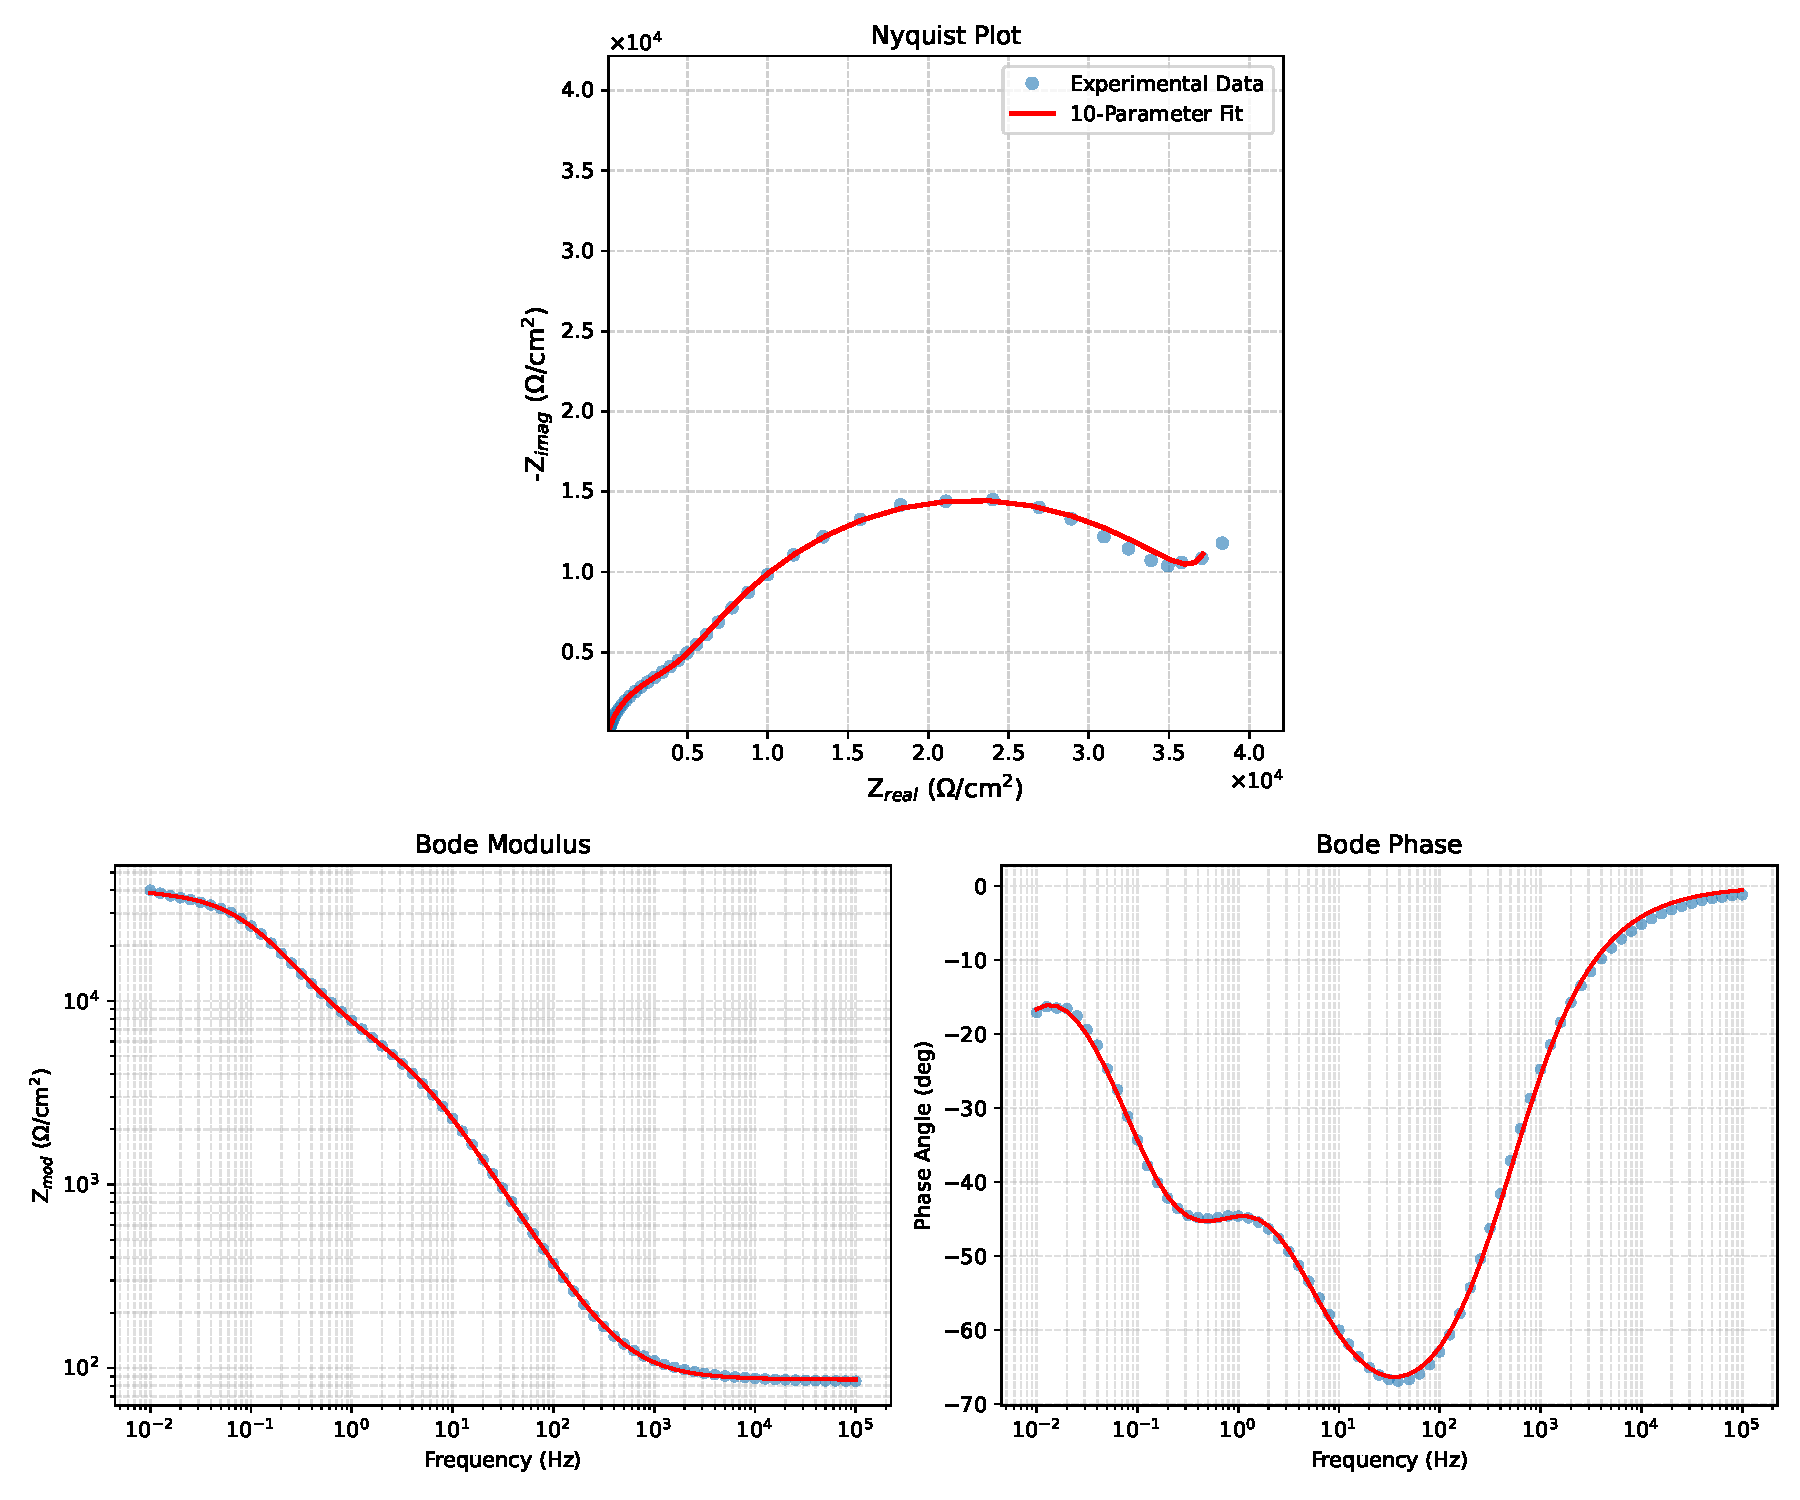
\includegraphics[width=0.7\textwidth]{plots_Cauvel_3_BTA_72H.pdf}
    \captionof{figure}{EIS Fit Results for Cauvel\_3\_BTA\_72H}
\end{center}

\newpage
\section*{Analysis Results: 168H}
\begin{center}
    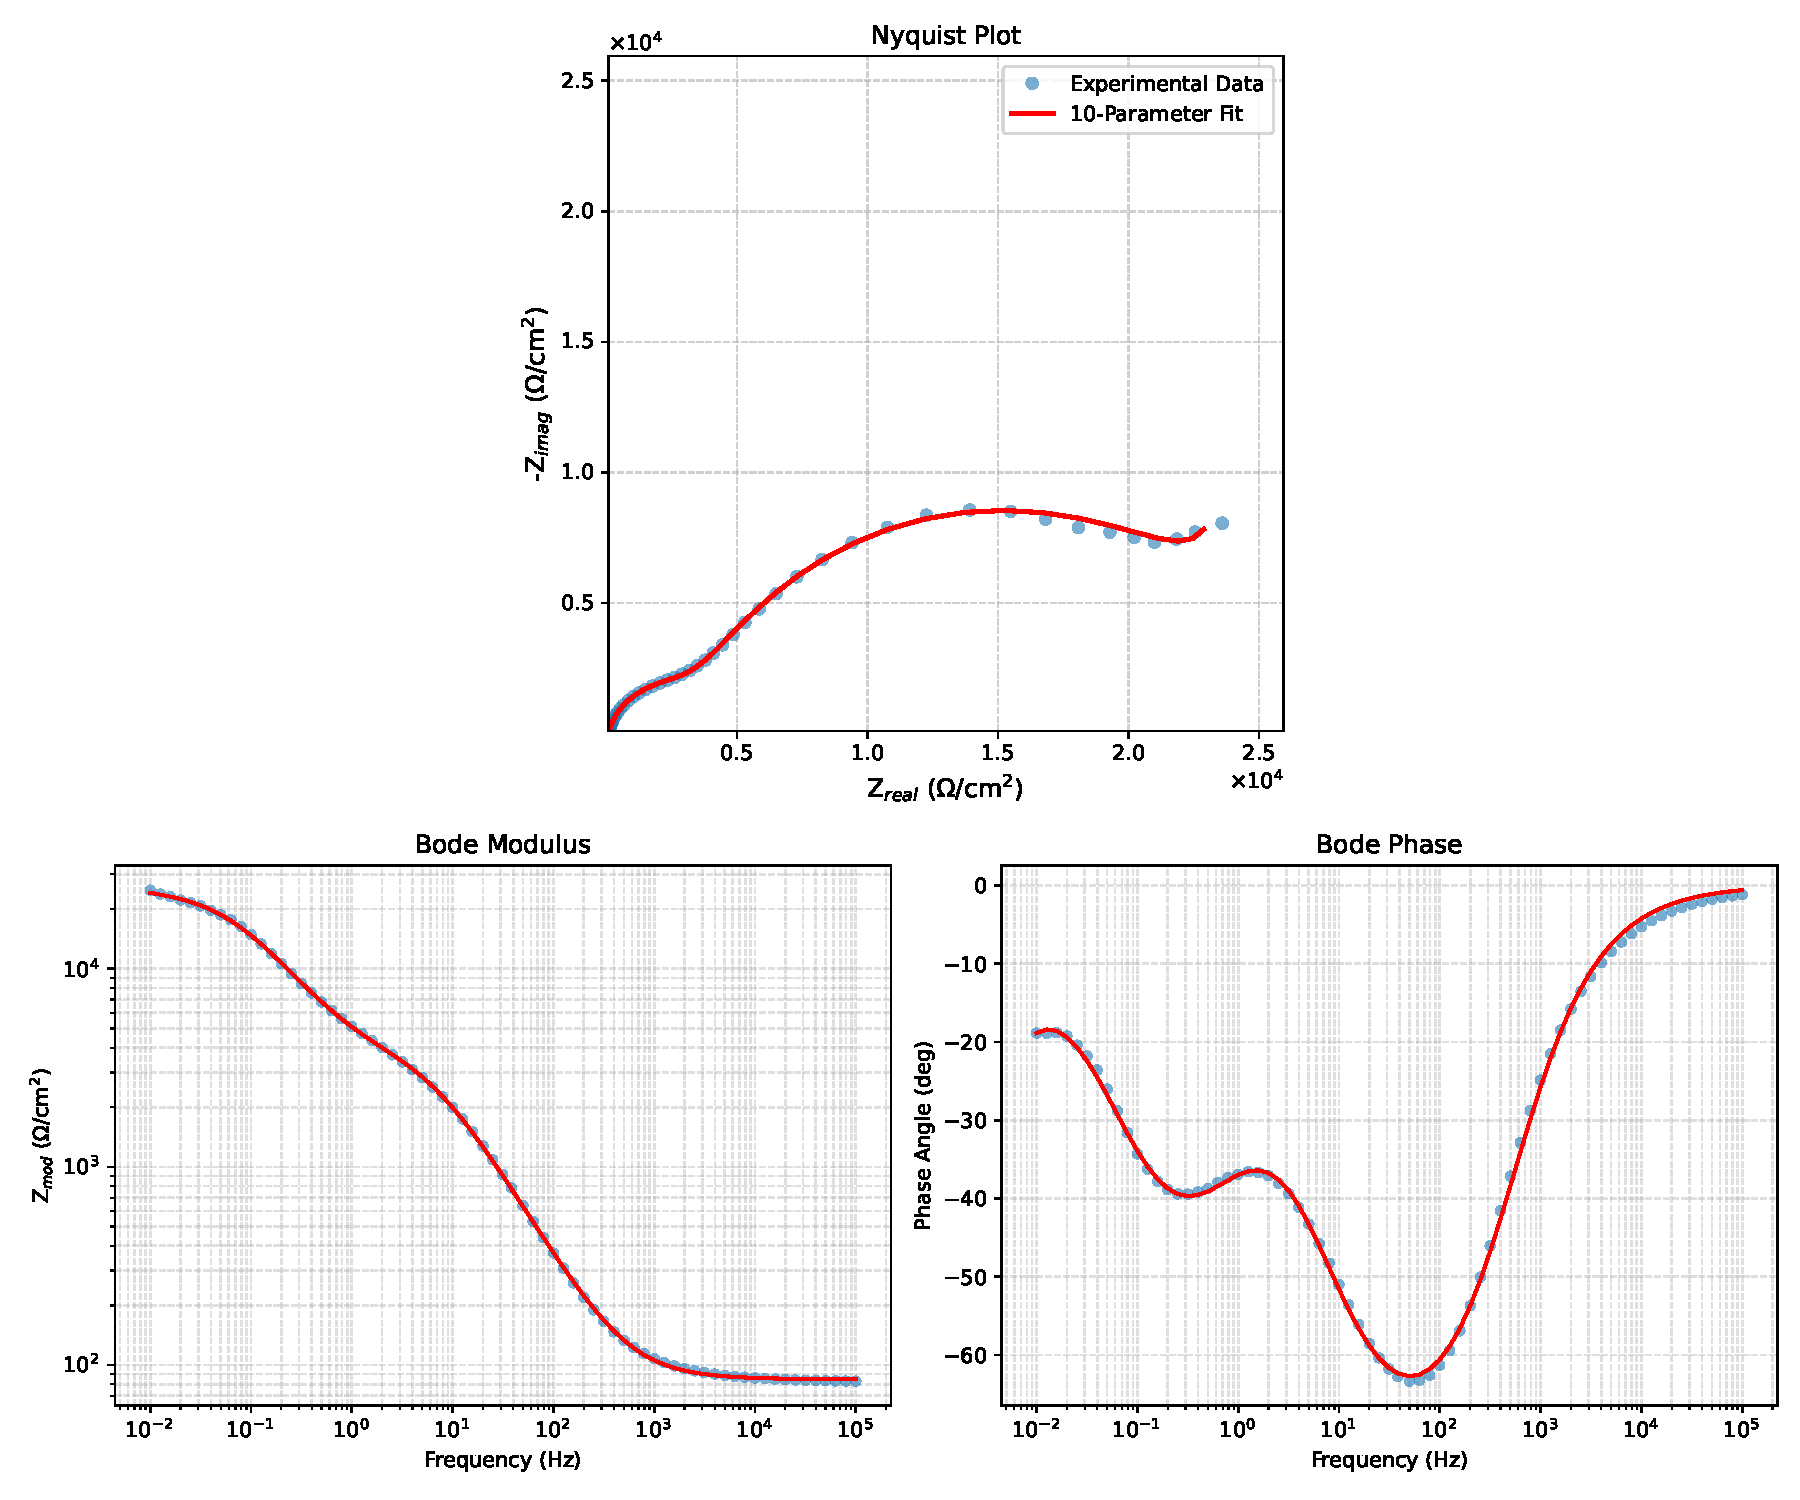
\includegraphics[width=0.7\textwidth]{plots_Cauvel_3_BTA_168H.pdf}
    \captionof{figure}{EIS Fit Results for Cauvel\_3\_BTA\_168H}
\end{center}


\end{document}
